S Bre{ß} and others developed CoGaDB architecture to be highly efficient and modularized as shown in top-down approach in Figure \ref{fig:cogadbarch}.
As most DBMSs, CoGaDB provides SQL frontend interface which can be used to write SQL language queries and launch it to get results from database. The SQL interface converts the provided language query into abstract syntax tree which is then pushed to logical optimizer module after being converted into a logical plan. Then, CoGaDB's logical optimizer applies pre-defined optimization policies on the logical plan such as pushing down selections, cross products resolution and reviewing join conditions. After this, the more efficient logical query plan is provided to HyPE for processing.
\begin{figure}
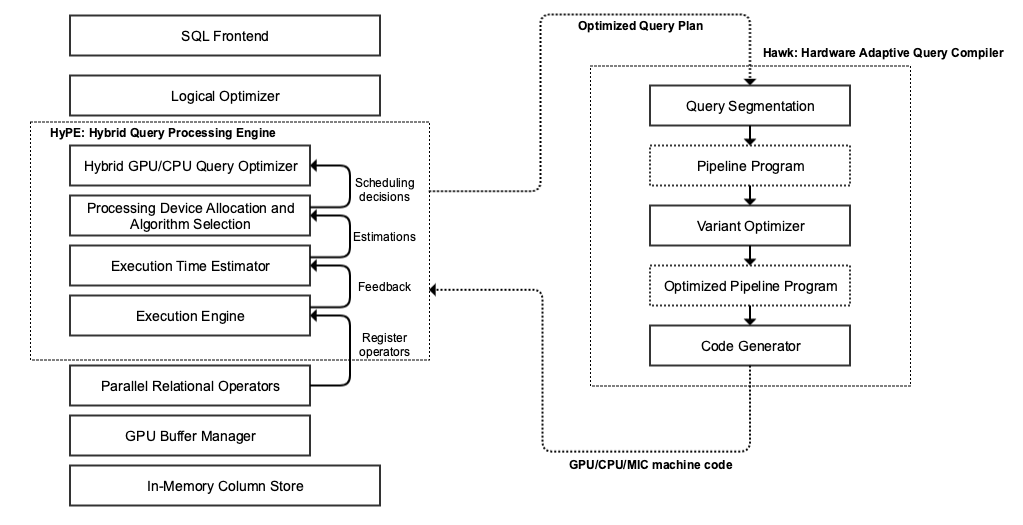
\includegraphics[width=\textwidth]{cogadb_hawk_architecture}
\caption{The architecture of CoGaDB, adapted from \cite{cogadb_hawk} and \cite{cogadb_manual}}
\label{fig:cogadbarch}
\end{figure}